\section{开闭集与邻近关系}
\label{sec:metric-open-closed}

度量给出的是两点之间的数值。要谈“一点附近”“集合的边缘”“用少数点代表整个空间”，需要把这些数值组织成关于集合的判断。本节先用开球描述一点附近允许怎样移动，再由此定义开集与闭集，接着用内部、闭包与边界刻画点相对集合的位置，最后讨论能否用可数个代表点逼近空间中的每一点。本节始终固定一个度量空间$(X,d)$。

\subsection{开球与邻域}
\label{sec:metric-balls}

在实轴上，“$x$离$a$不到$r$”就是$x\in(a-r,a+r)$。一般度量空间中没有区间，但同样可以把与中心距离小于$r$的点收集起来。

\begin{definition}[开球与邻域]
\label{def:metric-open-ball}
对$a\in X$与$r>0$，集合$B(a,r)=\{x\in X:d(x,a)<r\}$称为以$a$为中心、$r$为半径的\term{开球}（open ball）。若$V\subseteq X$包含某个开球$B(a,r)$，就称$V$是$a$的一个\term{邻域}（neighborhood）。
\end{definition}

定义中的不等号是严格的，半径必须为正，因此中心本身总在球内。邻域只要求在$a$周围留出一个球的余量：实轴上的$[0,1]$是$1/2$的邻域，因为$B(1/2,1/2)=(0,1)\subseteq[0,1]$；它却不是$0$的邻域，因为每个$(-r,r)$都含有负数。

\paragraph{球的形状由度量决定}
“球”只是一个名称，它的形状完全由度量决定。在$\mathbb R^2$中，单位球$B(\bm 0,1)$在$d_2$下是圆盘内部，在$d_\infty$下是边与坐标轴平行的正方形内部$\{\bm x:|x_1|<1,|x_2|<1\}$，在$d_1$下是以四个坐标轴上的点$(\pm1,0)$、$(0,\pm1)$为顶点的菱形内部。由$\lVert\bm x\rVert_\infty\leq\lVert\bm x\rVert_2\leq\lVert\bm x\rVert_1$，三个单位球依次嵌套：$d_1$的菱形最小，$d_\infty$的正方形最大，见图~\ref{fig:metric-unit-balls}。在离散度量下，半径不超过$1$的球只含中心一个点，与“圆”毫无相似之处。

\begin{figure}[!htbp]
  \centering
  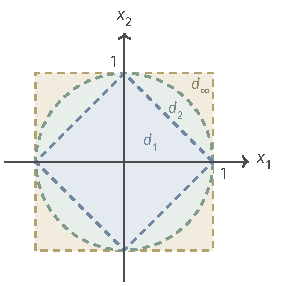
\includegraphics[width=48.055mm]{figures/02-abstract-mathematics/01-metric-and-measure/tikz/c1-unit-balls/figure.pdf}
  \caption{$\mathbb R^2$中以原点为中心的单位开球在三种度量下的形状。最内的菱形是$d_1$单位球，中间的圆盘是$d_2$单位球，最外的正方形是$d_\infty$单位球；虚线边界不属于开球。嵌套顺序对应$\lVert\bm x\rVert_\infty\leq\lVert\bm x\rVert_2\leq\lVert\bm x\rVert_1$：距离读数越大，同一半径的球越小。}
  \label{fig:metric-unit-balls}
\end{figure}

\paragraph{球内每点都有更小的球}
若$y\in B(a,r)$，令$\rho=r-d(y,a)>0$。对任意$z\in B(y,\rho)$，三角不等式给出$d(z,a)\leq d(z,y)+d(y,a)<\rho+d(y,a)=r$，所以
\begin{equation}
\label{eq:metric-ball-inside-ball}
  B(y,\rho)\subseteq B(a,r).
\end{equation}
也就是说，开球中的每一点自己也有一个留在球内的小球，这是下一小节证明“开球是开集”的依据。

\paragraph{相对开球}
设$A\subseteq X$配备子空间度量。为区分所在空间，把$A$中的开球记为$B_A(a,r)$，把$X$中的开球记为$B_X(a,r)$。对$a\in A$与$r>0$，
\begin{equation}
\label{eq:metric-relative-ball}
  B_A(a,r)=A\cap B_X(a,r),
\end{equation}
因为两边都恰好由“属于$A$且与$a$的距离小于$r$”的点组成，而子空间中的距离数值与$X$中相同。取$A=[0,1]\subseteq\mathbb R$与端点$0$，当$0<r\leq1$时，$B_A(0,r)=[0,1]\cap(-r,r)=[0,r)$。于是$[0,1/2)$在$A$中是$0$的邻域，在$\mathbb R$中却不是。图~\ref{fig:metric-relative-ball}画出了这个交集。判断邻域时，必须先说明当前所在的空间。

\begin{figure}[!htbp]
  \centering
  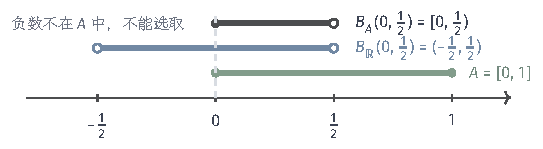
\includegraphics[width=91.934mm]{figures/02-abstract-mathematics/01-metric-and-measure/tikz/c1-relative-ball/figure.pdf}
  \caption{子空间中的相对开球。环境空间$\mathbb R$中的球$B_{\mathbb R}(0,r)=(-r,r)$（蓝色）伸到负半轴，而负数不属于子空间$A=[0,1]$（绿色）；二者的交集就是$A$中的球$B_A(0,r)=[0,r)$，它包含端点$0$。图中取$r=1/2$。}
  \label{fig:metric-relative-ball}
\end{figure}

\subsection{开集与闭集}
\label{sec:metric-open-sets}

邻域描述的是单个点。若一个集合是其中每一点的邻域，集合中的点无论在哪里，都可以向各个方向稍作移动而不离开它。

\begin{definition}[开集与闭集]
\label{def:metric-open-closed}
若对每个$x\in U$都存在$r>0$使$B(x,r)\subseteq U$，就称$U\subseteq X$为\term{开集}（open set）。若$X\setminus F$是开集，就称$F\subseteq X$为\term{闭集}（closed set）。
\end{definition}

半径可以随点改变，越靠近边缘的点可用的球越小。由式~\eqref{eq:metric-ball-inside-ball}，每个开球都是开集。空集没有需要检查的点，所以是开集；$X$包含它的每个球，所以也是开集。二者互为补集，因此它们同时也是闭集。

\begin{theorem}[开集与闭集的运算]
\label{thm:metric-open-operations}
任意多个开集的并是开集，有限多个开集的交是开集；任意多个闭集的交是闭集，有限多个闭集的并是闭集。
\end{theorem}

\begin{proof}
设$\{U_\alpha\}$是一族开集，$x\in\bigcup_\alpha U_\alpha$。则$x$属于某个$U_\beta$，存在$r>0$使$B(x,r)\subseteq U_\beta\subseteq\bigcup_\alpha U_\alpha$，所以并集是开集。

设$U_1,\dots,U_k$是开集，$x\in\bigcap_{i=1}^kU_i$。对每个$i$取$r_i>0$使$B(x,r_i)\subseteq U_i$，令$r=\min_ir_i$。由于只有有限个正数，$r>0$，而且$B(x,r)\subseteq B(x,r_i)\subseteq U_i$对每个$i$成立，所以$B(x,r)\subseteq\bigcap_iU_i$。

闭集的两条结论由补集关系得到：$X\setminus\bigcap_\alpha F_\alpha=\bigcup_\alpha(X\setminus F_\alpha)$是开集的并，$X\setminus\bigcup_{i=1}^kF_i=\bigcap_{i=1}^k(X\setminus F_i)$是有限个开集的交。
\end{proof}

证明中“有限”的作用在于取最小值时得到正数；对无限多个半径，下确界可能是零。例如每个$(-1/n,1/n)$都是$\mathbb R$中的开集，它们的交却是$\{0\}$，不是开集，因为$0$的每个球都含有非零数。同理，每个$[1/n,1]$都是闭集，它们的并$(0,1]$却不是闭集：补集$(-\infty,0]\cup(1,\infty)$在点$0$处没有留在其中的球。

\paragraph{开与闭不是互斥的两类}
“不开”不意味着“闭”。$X$与$\varnothing$既开又闭；实轴上的$[0,1)$既不开也不闭：$0\in[0,1)$没有留在其中的球，所以它不是开集；$1$在补集中，但每个$B(1,r)$都含有$[0,1)$中的点，所以补集不是开集。

\paragraph{子空间中的开集与闭集}
开与闭还取决于所在空间。由式~\eqref{eq:metric-relative-ball}可以把子空间中的开集化为环境空间的开集。

\begin{lemma}[子空间的开集与闭集]
\label{lem:metric-relative-open}
设$A\subseteq X$配备子空间度量。$U\subseteq A$是$A$中的开集，当且仅当存在$X$中的开集$V$使$U=A\cap V$；$F\subseteq A$是$A$中的闭集，当且仅当存在$X$中的闭集$C$使$F=A\cap C$。
\end{lemma}

\begin{proof}
若$U=A\cap V$且$V$在$X$中开，对$x\in U$取$r>0$使$B_X(x,r)\subseteq V$，则$B_A(x,r)=A\cap B_X(x,r)\subseteq A\cap V=U$，所以$U$在$A$中开。反过来，若$U$在$A$中开，对每个$x\in U$取$r_x>0$使$B_A(x,r_x)\subseteq U$，令$V=\bigcup_{x\in U}B_X(x,r_x)$。$V$是开球的并，在$X$中开；并且$A\cap V=\bigcup_{x\in U}B_A(x,r_x)$，它包含每个$x\in U$，又包含于$U$，所以等于$U$。

对闭集，$F$在$A$中闭当且仅当$A\setminus F$在$A$中开，即$A\setminus F=A\cap V$对某个$X$中的开集$V$成立；这又等价于$F=A\cap(X\setminus V)$，其中$X\setminus V$在$X$中闭。
\end{proof}

例如在子空间$A=[0,1]$中，$[0,1/2)=A\cap(-1,1/2)$与$(1/2,1]=A\cap(1/2,2)$都是开集，尽管它们在$\mathbb R$中都不是开集；$[0,1/2]=A\cap[-1,1/2]$是$A$中的闭集。$A$本身在$A$中既开又闭，这与它在$\mathbb R$中只闭不开并不矛盾。

\subsection{内部、闭包与边界}
\label{sec:metric-closure}

同一族开球还可以对单个点相对集合的位置分类：点可能深入集合内部，可能紧贴集合，也可能同时贴着集合与它的补集。

\begin{definition}[内部、闭包与边界]
\label{def:metric-closure}
设$A\subseteq X$。若存在$r>0$使$B(x,r)\subseteq A$，称$x$为$A$的内点，全部内点组成$A$的\term{内部}（interior），记作$A^\circ$。若对每个$r>0$都有$B(x,r)\cap A\neq\varnothing$，称$x$为$A$的闭包点，全部闭包点组成$A$的\term{闭包}（closure），记作$\overline A$。若对每个$r>0$，$B(x,r)$既与$A$相交又与$X\setminus A$相交，称$x$为$A$的边界点，全部边界点组成$A$的\term{边界}（boundary），记作$\partial A$。
\end{definition}

三个定义的区别在量词：内点要求“存在一个球”留在集合内，闭包点要求“每个球”都碰到集合，边界点要求“每个球”同时碰到两侧。按定义$A^\circ\subseteq A\subseteq\overline A$，因为$x\in A$时每个球都含有$x$本身。图~\ref{fig:metric-interior-closure-boundary}画出了三类位置。

\begin{figure}[!htbp]
  \centering
  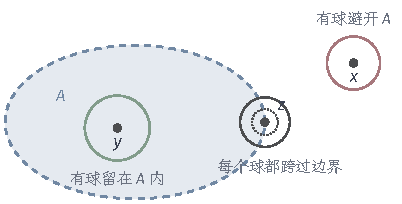
\includegraphics[width=68.104mm]{figures/02-abstract-mathematics/01-metric-and-measure/tikz/c1-interior-closure-boundary/figure.pdf}
  \caption{点相对集合$A$（浅蓝区域，虚线边界不属于$A$）的三种位置。内点$y$有一个完全落在$A$中的球；边界点$z$的每个球都同时碰到$A$与补集，它在$\overline A$中却可以不属于$A$；点$x$有一个完全避开$A$的球，所以$x\notin\overline A$。}
  \label{fig:metric-interior-closure-boundary}
\end{figure}

\paragraph{边界等于闭包去掉内部}
$x\notin A^\circ$恰好表示没有球留在$A$中，即每个球都碰到$X\setminus A$。所以边界点就是“既是闭包点、又不是内点”的点：
\begin{equation}
\label{eq:metric-boundary}
  \partial A=\overline A\setminus A^\circ.
\end{equation}
在$\mathbb R$中，$(0,1)$与$[0,1]$的内部都是$(0,1)$，闭包都是$[0,1]$，边界都是$\{0,1\}$：边界点可以属于集合，也可以不属于集合。有理数集$\mathbb Q$的情形更极端：每个区间都同时含有有理数和无理数，所以$\mathbb Q^\circ=\varnothing$、$\overline{\mathbb Q}=\mathbb R$、$\partial\mathbb Q=\mathbb R$。

\paragraph{闭包是闭集}
若$x\notin\overline A$，存在$r>0$使$B(x,r)\cap A=\varnothing$。对$y\in B(x,r)$，取$\rho=r-d(x,y)$，由式~\eqref{eq:metric-ball-inside-ball}，$B(y,\rho)\subseteq B(x,r)$也避开$A$，所以$y\notin\overline A$。于是$X\setminus\overline A$包含其每一点的一个球，是开集。由此得到：$A$是闭集当且仅当$A=\overline A$。若$A$闭而$x\notin A$，则$x$属于开集$X\setminus A$，有一个避开$A$的球，$x\notin\overline A$，故$\overline A\subseteq A$；反过来，$A=\overline A$时$A$就是闭集。对内部有对称的结论：$A^\circ$是开集，$A$开当且仅当$A=A^\circ$；论证只需把“避开$A$”换成“留在$A$内”。

\paragraph{点到集合的距离}
“每个球都碰到$A$”还可以写成一个数值条件。对非空集合$A$，定义点$x$到$A$的距离
\begin{equation}
\label{eq:metric-distance-to-set}
  d(x,A)=\inf_{a\in A}d(x,a).
\end{equation}
它是有限的非负数，因为任取$a_0\in A$都有$0\leq d(x,A)\leq d(x,a_0)$。由下确界的定义，对任意$\varepsilon>0$都有$a\in A$使$d(x,a)<d(x,A)+\varepsilon$。

\begin{lemma}[距离为零与闭包]
\label{lem:metric-distance-closure}
设$A\subseteq X$非空。则$x\in\overline A$当且仅当$d(x,A)=0$。
\end{lemma}

\begin{proof}
若$d(x,A)=0$，对每个$r>0$，由下确界的逼近性质有$a\in A$使$d(x,a)<r$，即$B(x,r)\cap A\neq\varnothing$，所以$x\in\overline A$。反过来，若$x\in\overline A$，对每个$r>0$有$a\in B(x,r)\cap A$，于是$d(x,A)\leq d(x,a)<r$；$r$任意，故$d(x,A)=0$。
\end{proof}

距离为零只说明$x$紧贴$A$，并不说明$x\in A$：$d(0,(0,1))=0$，而$0\notin(0,1)$。下确界也不一定由$A$中的某个“最近点”达到：$d(2,(0,1))=1$，但对每个$a\in(0,1)$都有$|2-a|>1$。什么条件能保证最近点存在，要等到第~\ref{sec:metric-continuous-maps}节讨论紧致集上的连续函数时回答。

\subsection{稠密集与可分空间}
\label{sec:metric-separable}

计算中只能存储有理数，却可以把任何实数逼近到任意精度。这说明一个较小的集合可以“代表”整个空间：它不必包含每一点，但必须与每一点任意接近。

\begin{definition}[稠密集与可分空间]
\label{def:metric-separable}
若$\overline D=X$，就称$D\subseteq X$在$X$中\term{稠密}（dense）。若$X$存在可数的稠密子集，就称$X$是\term{可分}（separable）的。
\end{definition}

按闭包的定义，$D$稠密等价于每个开球$B(x,r)$都与$D$相交：无论指定哪个位置$x$和哪个精度$r$，$D$中总有一点在该精度内代表$x$。可分性的要求更强，它要求同一套可数个代表点服务所有位置和所有精度。可数集合的概念见\BookChapterRef{chap:cardinality}{卷一“基数”章}。

\paragraph{实轴与离散空间}
在通常距离下，任意区间$(x-r,x+r)$都含有有理数，所以$\mathbb Q$在$\mathbb R$中稠密，而$\mathbb Q$可数，$\mathbb R$是可分的；同理，$\mathbb Q^d$在$(\mathbb R^d,d_2)$中稠密，因为对每个坐标取误差小于$r/\sqrt d$的有理数，所得点的欧氏误差小于$r$。另一方面，在不可数集合（例如$\mathbb R$本身）上取离散度量，每个单点集都是开球$B(x,1/2)=\{x\}$，稠密集必须与每个单点相交，只能是全空间，因而不可数，空间不可分。两个例子使用同一个底集$\mathbb R$，只因度量不同，可分性就不同。可分也不意味着空间本身可数：$\mathbb R$不可数，却有可数稠密子集$\mathbb Q$。

图~\ref{fig:metric-unit-balls}中的球形状和本节的相对球已经表明，邻近结构由度量和所在空间共同决定。下一节用这套邻近结构研究点列：给定精度后，点列的项最终能否都落进某个球内。
